% APA7
% https://ctan.org/pkg/apa7
\documentclass[stu,12pt,a4paper,biblatex,floatsintext]{apa7}

% Improves full justification and other micro-typographic aspects
% https://ctan.org/pkg/microtype
\usepackage{microtype}

% Times-like fonts
% https://ctan.org/pkg/newtx
% https://ctan.org/pkg/newtxtt
\usepackage{newtx, newtxtt}

% Avoid widows
% https://ctan.org/pkg/nowidow
\usepackage[all]{nowidow}

% Tabulars with adjustable-width columns
% https://ctan.org/pkg/tabularx
\usepackage{tabularx}

% For centering columns with `tabularx`
% Taken from: https://tex.stackexchange.com/a/89932
\newcolumntype{Y}{>{\centering\arraybackslash}X}

% For creating tabular cells that span multiple rows
% https://ctan.org/pkg/multirow
\usepackage{multirow}

% Extra break points for URLs
% Particularly useful for long URLs
% https://ctan.org/pkg/xurl
\usepackage{xurl}

% Use graphics from `./graphics/`
% https://ctan.org/pkg/graphicx
\graphicspath{ {./graphics/} }

% Use references from `references.bib`
% https://ctan.org/pkg/biblatex
\addbibresource{references.bib}

% Preamble from `apa7`
% See the `apa7` documentation for more commands
\title{Title}
\author{Author}
\affiliation{Affiliation}
\course{Course}
\professor{Professor}
\duedate{Due date}

\begin{document}

% From the `apa7` documentation:
% "The `\maketitle` command formats the document title, page headers, author list,
% author affiliations, Author Note (if provided), abstract according to whether `jou`,
% `man`, `stu`, or `doc` mode has been specified."
\maketitle

This is some introductory text.

\section{Citations}

\subsection{Parenthetical Citations}

This is a citation \parencite{example1970}.

This is a citation with page numbers \parencite[1-2]{example1970}.

This is a citation with some extra text \parencite[Appendix A]{example1970}. Here is another one \parencite[ch. 1 p. 1]{example1970}.

\subsection{Narrative Citations}

\textcite{example1970} shows that this is a narrative citation.

The options for parenthetical citations can be applied to narrative citations as well: \textcite[1-2]{example1970}; \textcite[Appendix A]{example1970}.

\section{Enumerations}

The following is a seriation: \begin{seriate}
	\item Item 1
	\item Item 2
	\item Item 3
\end{seriate}.

The following is an enumeration: \begin{APAenumerate}
	\item Item 1
	\item Item 2
	\item Item 3
\end{APAenumerate}.

The following is an itemization: \begin{APAitemize}
	\item Item 1
	\item Item 2
	\item Item 3
\end{APAitemize}.

\section{Tables}

\begin{table}[H]
	\caption{A basic table}
	\label{table:example1}
	\centering
	\begin{tabular}{r*{4}{c}}
		\toprule
		      & Column 1 & Column 2 & Column 3 \\
		\midrule
		Row 1 & A        & B        & C        \\
		Row 2 & A        & B        & C        \\
		\bottomrule
	\end{tabular}
\end{table}

\begin{table}[H]
	\caption{A more complex table using \textnormal{\texttt{\textbackslash tabularx}}, \textnormal{\texttt{\textbackslash multirow}} and \textnormal{\texttt{\textbackslash multicolumn}}}
	\label{table:example2}
	\centering
	\begin{tabularx}{0.75\textwidth}{*{3}{Y}c}
		\toprule
		\multicolumn{3}{c}{Header 1} & \multirow{2}{*}{Header 2}                \\
		\cmidrule(r{0.5em}){1-3}
		Column 1                     & Column 2                  & Column 3     \\
		\midrule
		A                            & B                         & C        & D \\
		A                            & B                         & C        & D \\
		\bottomrule
	\end{tabularx}
\end{table}

\section{Graphics}

This is an image:

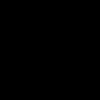
\includegraphics{example}

This is the same image, but included using \texttt{\textbackslash fitbitmap}:

\fitbitmap{example}

\printbibliography

\end{document}
